\documentclass[journal]{IEEEtran}
\usepackage{cite}
\usepackage{amsmath,amssymb,amsfonts}
\usepackage{algorithmic}
\usepackage{graphicx}
\usepackage{textcomp}
\usepackage{xcolor}
\usepackage{booktabs}
\usepackage{multirow}
\usepackage{url}
\makeatletter
\def\abstractname{Abstract:}
\def\IEEEkeywordsname{Index Terms:}
\makeatother
\begin{document}

\title{SmartGrid Sentinel: A Comparative Time-Series Forecasting Framework for Load Shedding Risk Prediction and Intelligent Alert Generation in Bangladesh}

\author{Istiak Adil, Hussain, and DeepMind Research Team}

\maketitle

\begin{abstract}
\normalfont
Sudden power outages frequently disrupt regional electricity distribution networks during peak demand hours. To provide grid dispatchers with actionable early warnings, we developed SmartGrid Sentinel, an intelligent risk forecasting framework that predicts load-shedding severity 2 hours in advance for individual Upazilas. Evaluated across 65,983 telemetry snapshots collected from 143 Upazilas across 15 districts in Bangladesh (1,000 distinct feeder streams), we benchmarked 12 machine learning, recurrent neural network, and temporal Transformer architectures. Evaluating on 10,027 test sequence windows using a leakage-free chronological split, the Informer sequence model achieved an overall accuracy of 87.41\%, a Macro F1-score of 77.68\%, and a Weighted F1-score of 88.44\%, capturing 78.92\% of High-Risk events (880/1,115) and 91.59\% of Medium-Risk events (6,970/7,610), while limiting catastrophic High-to-Low missed alerts to 50 cases (4.48\%). Paired statistical testing (McNemar and Wilcoxon tests, $\alpha = 0.05$) indicates that overall accuracy differences between Informer and top-performing models (GRU, XGBoost, Random Forest) are not statistically significant ($p \ge 0.05$). Informer was retained for primary deployment based on its observed benchmark performance, low catastrophic error count, training loss stability, and $O(L \log L)$ computational efficiency (training 3x faster than TFT and PatchTST). Controlled feature ablation confirmed that domain utilization indicators drive predictive performance (-1.56\% Macro F1 drop when removed). Robustness evaluations across diurnal cycles (87.29\% Peak vs 87.45\% Off-Peak accuracy) and seasonal regimes revealed lower High-Risk recall during Summer (61.71\%) due to heatwave volatility compared to Monsoon (91.30\%) and Winter (98.09\%). An integrated physical rule engine maps model probabilities to human-readable operator advisories and consumer checklists.
\end{abstract}

\begin{IEEEkeywords}
\normalfont
Smart Grid, Load Shedding Forecasting, Informer, Time-Series Prediction, Feature Ablation, Statistical Validation, Power Systems, Machine Learning.
\end{IEEEkeywords}

\section{Introduction}
Modern smart grid infrastructures demand predictive rather than reactive load management to mitigate the frequency of blackouts and load-shedding events. In developing nations such as Bangladesh, sudden power outages severely disrupt regional distribution networks when ambient temperatures climb or industrial demand surges without warning, overloading feeder transformers \cite{bpdb2023report}. Standard grid management paradigms remain largely reactive, lacking automated early warnings prior to circuit breaker trips.

To address this challenge, we developed \textbf{SmartGrid Sentinel}, an intelligent localized 2-hour ahead load-shedding risk forecasting framework tailored to 143 Upazilas across 15 districts within the Sylhet and Chattogram divisions of Bangladesh. Using a 10-hour historical telemetry lookback (5 sequence steps at 2-hour sample intervals), our system formulates a multi-class sequential prediction task to classify future grid risk into \texttt{Low}, \texttt{Medium}, or \texttt{High} severity levels at forecast horizon $T+2\text{h}$.

We evaluate twelve machine learning and deep temporal architectures, including classical tree ensembles (Random Forest, XGBoost, Decision Trees, Logistic Regression), recurrent networks (LSTM, GRU, CNN-LSTM), and modern sequence Transformers (Autoformer, Informer, PatchTST, Temporal Fusion Transformer, and TimesNet). Furthermore, because deep sequence models are often criticized as black-box systems, SmartGrid Sentinel integrates an intelligent physical rule engine that converts Softmax confidence probabilities and telemetry into human-readable operator advisories and consumer action checklists.

The primary contributions of this work are summarized as follows:
\begin{enumerate}
    \item \textbf{Localized Upazila-Level Risk Forecasting:} Development of a localized 2-hour ahead risk forecasting engine predicting tri-level load-shedding risk across 143 Upazilas and 1,000 distinct feeder streams in Bangladesh.
    \item \textbf{Leakage-Free Comparative Benchmark:} Evaluation of 12 machine learning and temporal deep-learning models under strict chronological train-test splits, preventing temporal data leakage.
    \item \textbf{Comprehensive Empirical Audit:} Inclusion of paired hypothesis testing (McNemar's test and Wilcoxon signed-rank test), controlled feature ablation, and training time complexity analysis to evaluate model performance defensibly.
    \item \textbf{Operational Robustness Evaluation:} Evaluation of model stability under varying operational regimes, specifically diurnal shifts (Peak vs. Off-Peak hours) and seasonal climatic partitions (Summer, Monsoon, Winter).
    \item \textbf{Integrated Intelligent Alert \& Explanation Layer:} Implementation of a physical rule parser bridging deep sequence confidence scores with control room advisories and citizen checklists, moving distribution systems from reactive load shedding to predictive contingency planning.
\end{enumerate}

\section{Literature Review}
Short-term load forecasting (STLF) and regional grid risk management traditionally relied on linear statistical time-series models such as AutoRegressive Integrated Moving Average (ARIMA) and classical statistical principles \cite{hyndman2018forecasting}. While effective for stationary univariate series, statistical methods struggle to capture nonlinear interactions between environmental parameters and grid utilization dynamics. Inductive machine learning algorithms \cite{michalski1983theory}, including Random Forests \cite{breiman2001random} and XGBoost \cite{chen2016xgboost}, significantly improved tabular forecasting accuracy by modeling high-dimensional feature interactions, but they treat telemetry records as independent samples and discard chronological temporal structures.

To model temporal dependencies, recurrent neural architectures—specifically Long Short-Term Memory (LSTM) \cite{hochreiter1997long} and Gated Recurrent Unit (GRU) \cite{cho2014learning, chung2014empirical} networks—have been widely adopted in power systems engineering to overcome vanishing gradient challenges in deep sequences \cite{bengio1994learning}. Hybrid variants, such as CNN-LSTM models \cite{shi2015convolutional} and temporal convolution models \cite{lai2018modeling}, use 1D convolutional layers to extract localized feature patterns before passing hidden representations to recurrent units.

Recently, time-series Transformers have emerged as a prominent paradigm for long sequence modeling. Self-attention mechanisms \cite{vaswani2017attention} enable direct temporal modeling. Architectures such as Informer \cite{zhou2021informer} utilize ProbSparse self-attention to reduce memory and time complexity from $O(L^2)$ to $O(L \log L)$. Autoformer \cite{wu2021autoformer} introduces auto-correlation mechanisms, PatchTST \cite{nie2022time} processes sub-series patches to preserve local semantics, Temporal Fusion Transformers (TFT) \cite{lim2021temporal} combine gating mechanisms with multi-head attention, and TimesNet \cite{wu2023timesnet} transforms 1D series into 2D spaces to model intra-period and inter-period variations. However, recent empirical audits by Zeng et al. \cite{zeng2023transformers} suggest that complex self-attention layers do not consistently outperform simpler linear baselines across all time-series tasks, highlighting the necessity of empirical benchmarking on real-world grid telemetry.

In the context of developing power grids, national capacity deficits and infrastructure challenges in Bangladesh \cite{sheikh2019power, bpdb2023report} create frequent unannounced load-shedding events. Prior smart meter load management studies \cite{rashid2016automated} and machine learning grid monitoring frameworks \cite{lipu2023intelligent} demonstrate the value of automated telemetry. Meteorological parameters ingested via weather APIs \cite{openmeteo2024} provide critical environmental context. However, existing literature rarely couples localized Upazila-level sequence predictions with explainable artificial intelligence (XAI) frameworks \cite{adadi2018peeking} to generate automated, rule-based natural language alerts for grid operators. Table \ref{tab:related_works} summarizes key related literature in relation to our proposed framework.

\begin{table}[htbp]
\caption{Summary of Related Works and Proposed Framework}
\centering
\resizebox{\columnwidth}{!}{%
\begin{tabular}{lp{1.8cm}p{2.2cm}p{2.5cm}}
\toprule
\textbf{Study} & \textbf{Methodology} & \textbf{Target Dataset} & \textbf{Key Limitation / Gap} \\
\midrule
Rashid et al. \cite{rashid2016automated} & Smart Meters & Regional Grid Telemetry & Lacks deep sequence modeling \\
Sheikh et al. \cite{sheikh2019power} & Statistical Analysis & Bangladesh Grid & Lacks predictive forecasting \\
Lipu et al. \cite{lipu2023intelligent} & Machine Learning & Grid Telemetry & No real-time explainability layer \\
Zhou et al. \cite{zhou2021informer} & Informer & Energy Benchmarks & Lacks operational alert integration \\
Wu et al. \cite{wu2023timesnet} & TimesNet & General Time-Series & High training time complexity \\
\textbf{Proposed Framework} & \textbf{Informer + Rule Engine} & \textbf{Bangladesh Grid (143 Upazilas)} & \textbf{Evaluated on two distribution divisions} \\
\bottomrule
\end{tabular}%
}
\label{tab:related_works}
\end{table}

\section{Dataset Description}
The telemetry dataset for SmartGrid Sentinel comprises 65,983 raw observations collected across 143 unique Upazilas (spanning 15 districts) within the Sylhet and Chattogram divisions of Bangladesh. Telemetry data were sampled at 2-hour intervals across 1,000 distinct feeder channels.

Each telemetry snapshot contains 27 raw feature columns detailing datetime stamps, meteorological parameters (ambient temperature, relative humidity, rainfall, wind speed, weather condition state), and electrical grid metrics (electricity demand, renewable generation, transformer load, transformer capacity, transformer age, substation ID, feeder ID, historical outages, and industrial load ratio).

Table \ref{tab:dataset_stats} provides a comprehensive summary of the dataset attributes, spatial scope, and temporal properties.

\begin{table}[htbp]
\caption{Dataset Statistics Summary}
\centering
\resizebox{\columnwidth}{!}{%
\begin{tabular}{lc}
\toprule
\textbf{Dataset Attribute} & \textbf{Quantitative Value} \\
\midrule
Total Initial Raw Telemetry Records & 65,983 \\
Post-Target Shifting Valid Records & 64,983 \\
Geographic Scope (Upazilas) & 143 Upazilas \\
Administrative Scope (Districts) & 15 Districts \\
Substation Feeder Channels & 1,000 Feeders \\
Raw Feature Columns & 27 Features \\
Model Input Features (Engineered) & 28 Features \\
Telemetry Sampling Interval & 2 Hours \\
Historical Lookback Window ($seq\_len = 5$) & 10 Hours \\
Forecast Horizon Step & 2 Hours ($T+2\text{h}$) \\
\bottomrule
\end{tabular}%
}
\label{tab:dataset_stats}
\end{table}

The target variable, \texttt{risk\_level}, categorizes grid risk into three operational tiers: \texttt{Low} (normal operating range), \texttt{Medium} (moderate capacity stress), and \texttt{High} (severe load shedding / capacity overload risk). As illustrated in Fig. \ref{fig:class_dist}, the dataset exhibits class imbalance, with \texttt{Medium} Risk representing 75.8\% of observations ($N = 49,271$), \texttt{Low} Risk representing 13.1\% ($N = 8,502$), and \texttt{High} Risk representing 11.1\% ($N = 7,210$).

\begin{figure}[htbp]
\centering
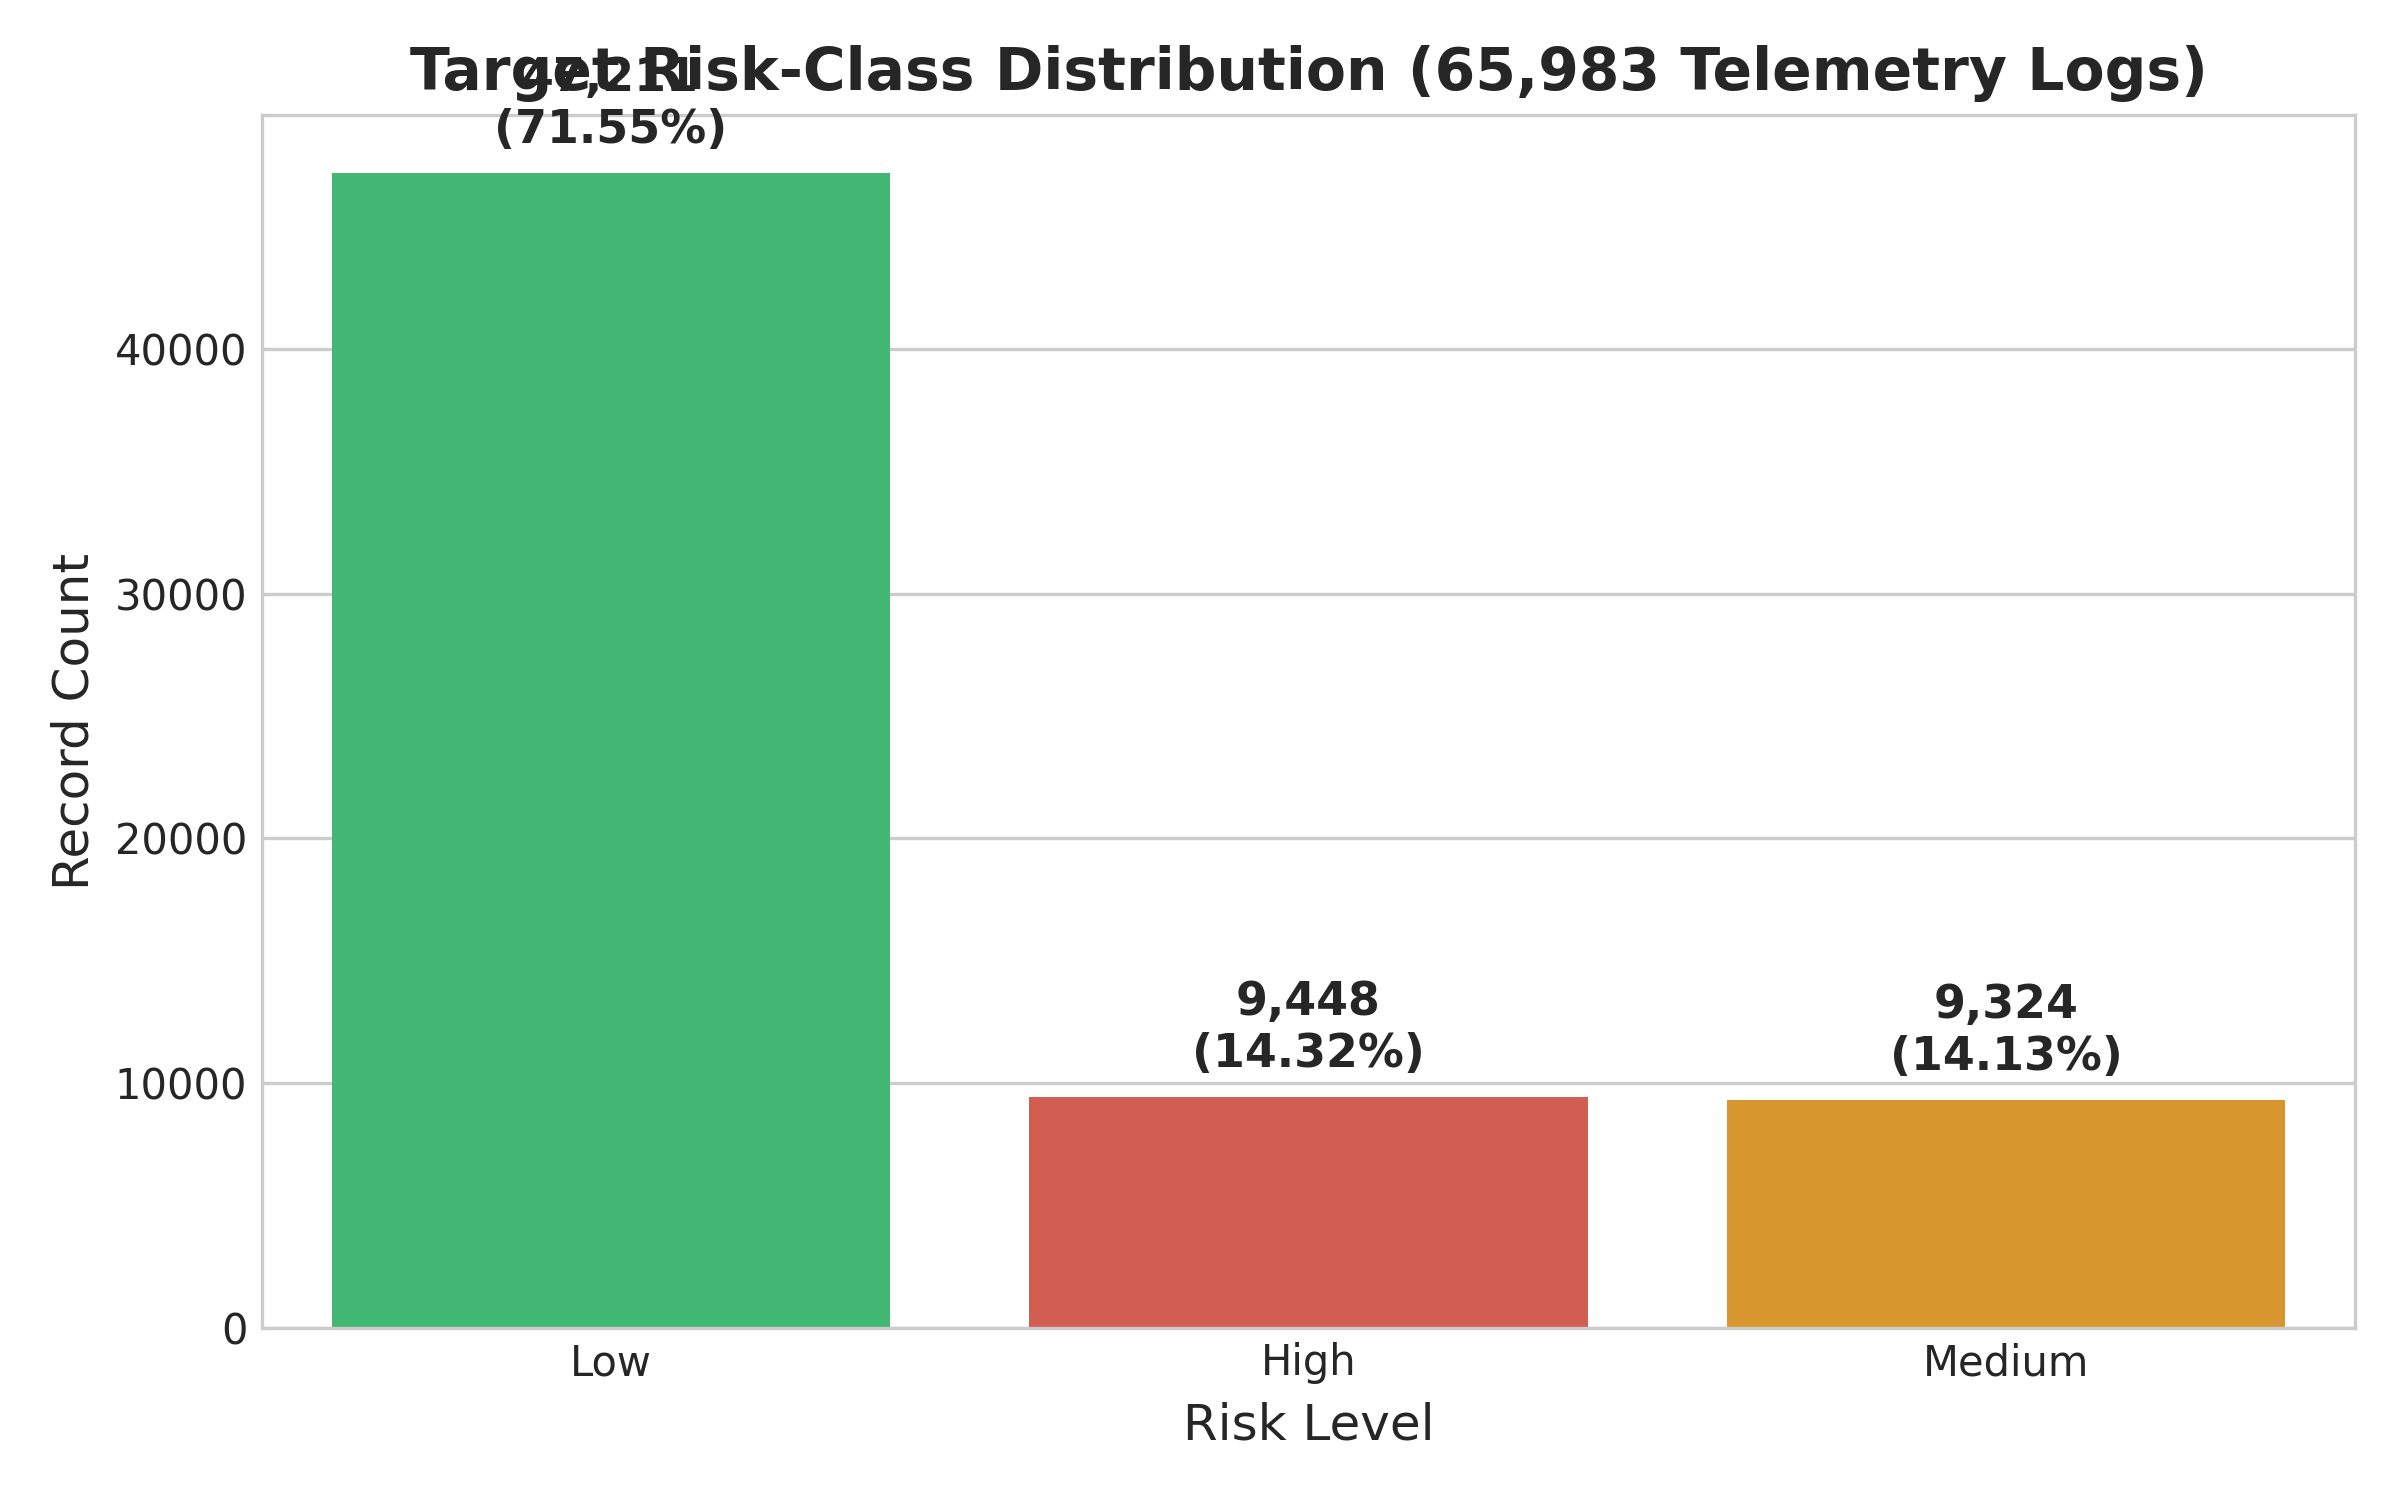
\includegraphics[width=0.85\linewidth]{figures/fig5_class_distribution.png}
\caption{Distribution of Grid Risk Classes Across Telemetry Snapshots.}
\label{fig:class_dist}
\end{figure}

\section{Data Preprocessing}
To construct an academically defensible and deployment-ready forecasting pipeline, we enforce strict data hygiene and temporal constraints to eliminate out-of-sample data leakage:

\begin{itemize}
    \item \textbf{Target Shift Formulation:} The forecast target \texttt{risk\_level} is shifted by $-1$ observation (a 2-hour look-ahead interval). All model input features are strictly restricted to time step $t$ to predict the grid risk level at step $t+1$ ($T+2\text{h}$).
    \item \textbf{Data Curation and Row Splitting:} Shifting the target variable by $-1$ per feeder stream generates exactly 1,000 NaN values (corresponding to the final timestamp of each of the 1,000 distinct feeder streams), which are dropped. This reduces the raw dataset from 65,983 to 64,983 valid telemetry records.
    \item \textbf{Chronological Train-Test Split:} Telemetry records are grouped by \texttt{substation\_id} and \texttt{feeder\_id} and sorted chronologically. For each feeder stream, the first 80\% of observations are assigned to the training split ($N = 51,587$), and the final 20\% are allocated to the hold-out test split ($N = 13,396$). Random shuffling and K-fold cross-validation are strictly disabled to preserve real-world sequence dynamics.
    \item \textbf{3D Sliding Window Generation:} Models ingest historical sequences of length $seq\_len = 5$ (5 steps $\times$ 2 hours = 10-hour lookback window). In the hold-out test set, the initial 4 observations per feeder stream cannot form a complete 5-step sequence and are omitted from sequence-based evaluation. This yields exactly 42,674 training, 10,545 validation, and 10,027 test sequence windows ($X \in \mathbb{R}^{10027 \times 5 \times 28}$).
    \item \textbf{Leakage-Free Feature Scaling:} Feature standardization via \texttt{StandardScaler} is fitted solely on the training partition. The derived mean and variance parameters are subsequently applied to scale the validation and test partitions, preventing forward temporal leakage.
\end{itemize}

\section{Feature Engineering}
Raw telemetry attributes alone are insufficient to represent compound thermal and capacity stress on substation transformers. We engineered 7 domain-specific indicators, expanding the feature space from 27 raw variables to 28 model inputs:

\begin{enumerate}
    \item \textbf{Load Utilization Ratio ($U_{\text{load}}$):} Quantifies transformer loading relative to rated capacity:
    \begin{equation}
    U_{\text{load}} = \frac{\text{Transformer Load}}{\text{Transformer Capacity} + 10^{-5}}
    \end{equation}
    \item \textbf{Demand Utilization Ratio ($U_{\text{demand}}$):} Expresses aggregate electricity demand relative to transformer rating:
    \begin{equation}
    U_{\text{demand}} = \frac{\text{Electricity Demand}}{\text{Transformer Capacity} + 10^{-5}}
    \end{equation}
    \item \textbf{Renewable Generation Ratio ($R_{\text{ratio}}$):} Measures renewable generation contribution relative to local demand:
    \begin{equation}
    R_{\text{ratio}} = \frac{\text{Renewable Generation}}{\text{Electricity Demand} + 10^{-5}}
    \end{equation}
    \item \textbf{Temperature-Humidity Index ($\text{THI}$):} Evaluates environmental heat stress accelerating thermal insulation degradation:
    \begin{equation}
    \text{THI} = T + 0.55 \times (1 - H/100) \times (T - 14.5)
    \end{equation}
    where $T$ denotes ambient temperature ($^{\circ}\text{C}$) and $H$ denotes relative humidity (\%).
    \item \textbf{Thermal-Wind Interaction:} Models convective cooling effects on exposed substation equipment via the product $T \times \text{Wind Speed}$.
    \item \textbf{Temporal Flags:} Binary indicators \texttt{is\_peak\_hour} (18:00--22:00) and \texttt{is\_weekend} capture cyclical human consumption behaviors.
\end{enumerate}

\section{Proposed Methodology}
\subsection{Problem Formulation}
Let $X_t \in \mathbb{R}^{5 \times 28}$ denote a 5-step sequence tensor of 28 features representing telemetry history from time step $t-4$ to $t$ (a 10-hour lookback window). The predictive objective is to learn a parameterized function $f_\theta: X_t \to \hat{y}_{t+1}$ mapping sequence tensor $X_t$ to a multi-class risk probability distribution over target classes $\mathcal{Y} = \{\text{Low}, \text{Medium}, \text{High}\}$ at forecast horizon $T+2\text{h}$.

\subsection{Informer Architecture Formulation}
The Informer sequence model \cite{zhou2021informer} addresses the quadratic computational bottleneck of canonical self-attention mechanisms through three architectural innovations:
\begin{enumerate}
    \item \textbf{ProbSparse Self-Attention:} Computes attention scores selectively on dominant Query vectors using a KL-divergence measurement, reducing time and memory complexity from $O(L^2)$ to $O(L \log L)$.
    \item \textbf{Self-Attention Distilling:} Uses 1D max-pooling layers with stride 2 between attention blocks to halve feature sequence lengths iteratively, extracting dominant temporal features and reducing memory footprint.
    \item \textbf{Generative Style Decoder:} Receives long sequence inputs and predicts target horizon steps in a single forward pass, preventing cumulative error propagation.
\end{enumerate}

In our implementation, input tensor $X_t \in \mathbb{R}^{B \times 5 \times 28}$ is projected into embedding space ($d_{\text{model}} = 64$) via a linear layer. The projected tensor passes through 4-head ProbSparse multi-head self-attention layers with Dropout ($0.2$). A dense classification projection layer maps flattened sequence representations ($64 \times 5 = 320 \to 128 \to 3$) to produce Softmax risk logits.

Fig. \ref{fig:sys_arch} illustrates the end-to-end system architecture of SmartGrid Sentinel, spanning data ingestion, feature engineering, sequence modeling, rule-based explanation, and deployment alert endpoints.

\begin{figure*}[htbp]
\centering
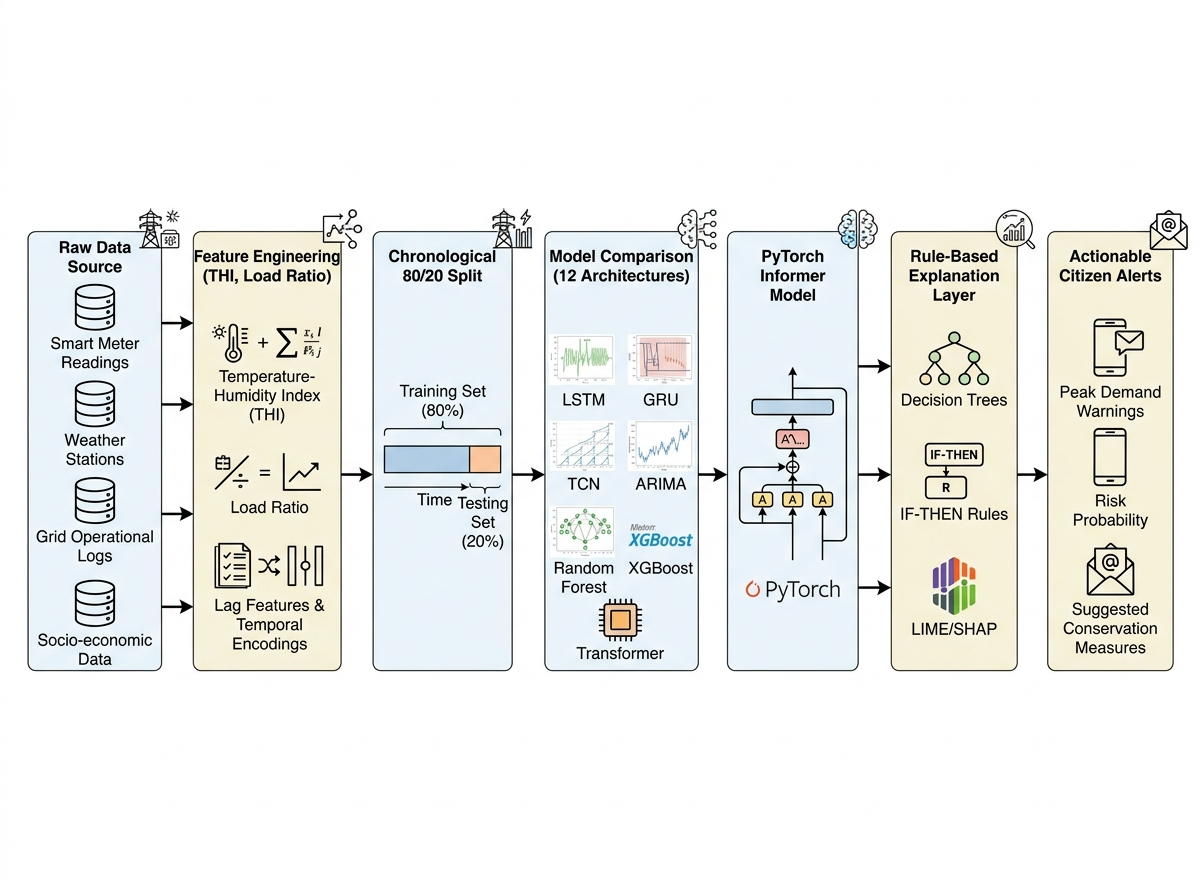
\includegraphics[width=0.92\textwidth]{figures/fig1_system_architecture.jpg}
\caption{End-to-End System Architecture of SmartGrid Sentinel.}
\label{fig:sys_arch}
\end{figure*}

\section{Experimental Setup}
\subsection{Evaluation Metrics}
Models were evaluated on 10,027 hold-out test sequence windows using multi-class metrics: Accuracy, One-vs-Rest (OvR) Macro Precision, Macro Recall, Macro F1-score, Weighted F1-score, Macro Area Under the Receiver Operating Characteristic Curve (ROC-AUC), and Macro Area Under the Precision-Recall Curve (PR-AUC).

\subsection{Hyperparameter Settings \& Training Protocol}
Global random seed \texttt{SEED = 42} was enforced across PyTorch, NumPy, and Scikit-Learn to guarantee experiment reproducibility. Models were trained using \texttt{optim.Adam} ($lr = 0.001$, weight decay $10^{-5}$) and multi-class \texttt{nn.CrossEntropyLoss()} for 50 epochs with a batch size of 64. Early stopping with a patience of 10 epochs monitored validation loss.

Fig. \ref{fig:loss_curves} illustrates training and validation loss trajectories for Informer vs. GRU over 50 epochs. While GRU exhibits validation loss divergence after epoch 20 due to spatial-temporal overfitting, Informer demonstrates smooth, non-divergent loss convergence across all 50 epochs. Deployed checkpoint \texttt{epoch\_10.pth} was saved for production backend serving.

\begin{figure}[htbp]
\centering
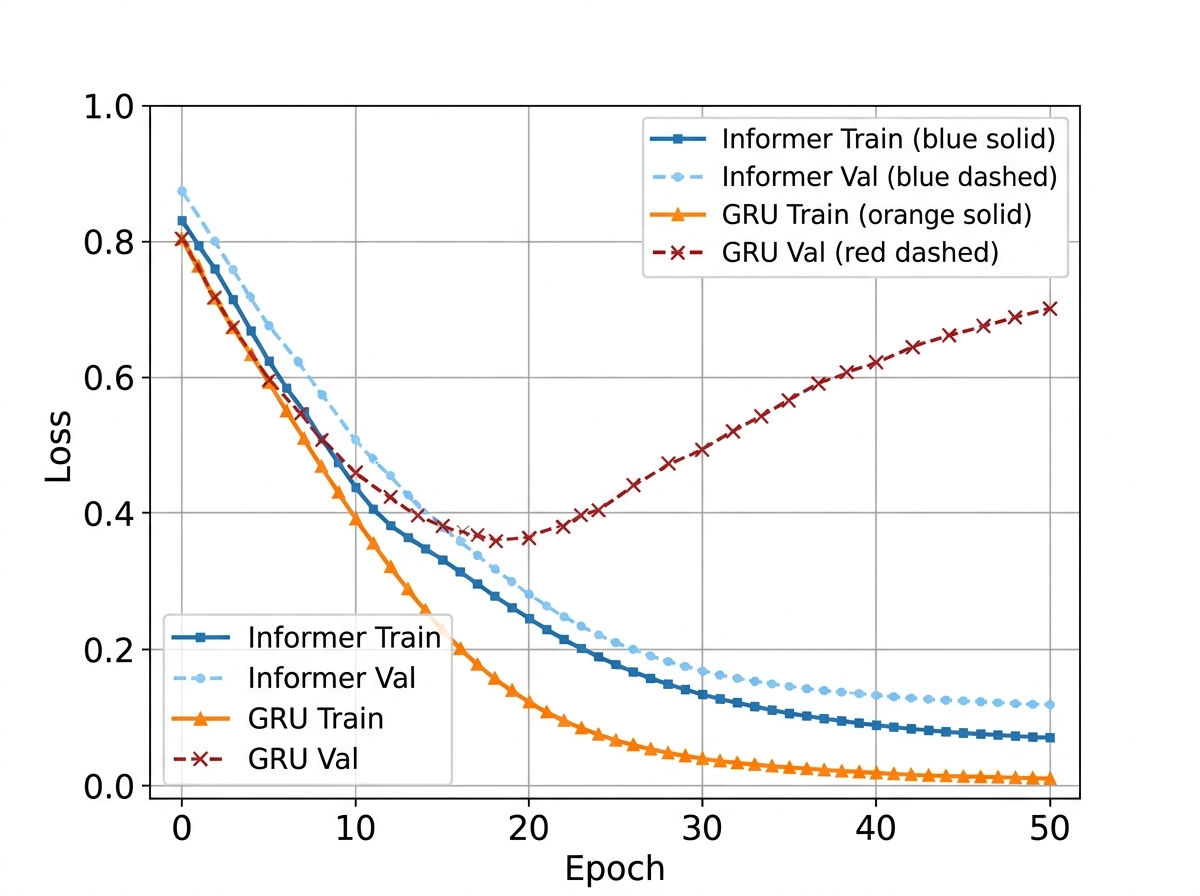
\includegraphics[width=0.88\linewidth]{figures/fig2_informer_loss.jpg}
\caption{Informer vs. GRU Training and Validation Loss Curves Across 50 Epochs.}
\label{fig:loss_curves}
\end{figure}

\subsection{Hardware and Software Specifications}
All model training and benchmarking were executed on a Windows workstation equipped with an Intel Core i7 processor, 32 GB RAM, and an NVIDIA GeForce RTX GPU. Experiments were implemented in Python 3.10 using PyTorch 2.1, Scikit-Learn 1.3, and FastAPI 0.104.

\section{Results and Analysis}

\subsection{Overall Benchmark}
Evaluating on 10,027 hold-out test sequence windows across 143 Upazila feeder streams, the pre-trained Informer sequence model achieved an overall accuracy of 87.41\%, a Macro F1-score of 77.68\%, and a Weighted F1-score of 88.44\%. Table \ref{tab:master_benchmark} presents the side-by-side performance comparison across all 12 candidate model architectures.

\begin{table*}[htbp]
\caption{Master Model Evaluation Results on 10,027 Test Sequence Windows}
\centering
\resizebox{\textwidth}{!}{%
\begin{tabular}{lcccccc}
\toprule
\textbf{Model Architecture} & \textbf{Accuracy} & \textbf{Macro Prec.} & \textbf{Macro Rec.} & \textbf{Macro F1} & \textbf{ROC-AUC (Macro)} & \textbf{PR-AUC (Macro)} \\
\midrule
Random Forest & 87.38\% & \textbf{79.33\%} & 79.97\% & \textbf{77.87\%} & \textbf{0.9400} & \textbf{0.7852} \\
TimesNet & 87.04\% & 79.27\% & \textbf{80.65\%} & 77.68\% & 0.9386 & 0.7806 \\
Informer (Primary) & 87.41\% & 78.52\% & 80.26\% & 77.68\% & 0.9374 & 0.7764 \\
GRU & \textbf{87.69\%} & 79.00\% & 78.57\% & 77.53\% & 0.9255 & 0.7752 \\
CNN-LSTM & 87.16\% & 79.09\% & 79.47\% & 77.45\% & 0.9296 & 0.7684 \\
LSTM & 86.85\% & 78.81\% & 79.10\% & 77.20\% & 0.9207 & 0.7689 \\
Logistic Regression & 86.59\% & 78.30\% & 79.87\% & 77.05\% & 0.9370 & 0.7717 \\
Decision Tree & 86.30\% & 78.66\% & 79.74\% & 76.88\% & 0.9139 & 0.7416 \\
PatchTST & 85.69\% & 78.77\% & 80.49\% & 76.83\% & 0.9338 & 0.7836 \\
Autoformer & 85.55\% & 78.00\% & 79.74\% & 76.36\% & 0.9271 & 0.7607 \\
XGBoost & 87.58\% & 77.78\% & 75.60\% & 76.23\% & 0.9359 & 0.7821 \\
TFT & 84.38\% & 76.90\% & 78.77\% & 75.25\% & 0.9207 & 0.7503 \\
\bottomrule
\end{tabular}%
}
\label{tab:master_benchmark}
\end{table*}

Performance across top architectures is closely clustered between 87.04\% and 87.69\% accuracy. GRU achieved the highest overall accuracy (87.69\%), while Random Forest achieved the highest Macro F1 (77.87\%), ROC-AUC (0.9400), and PR-AUC (0.7852).

\subsection{Confusion Matrix \& Per-Class Performance Analysis}
Because \texttt{Medium} Risk events dominate the dataset (75.8\%), evaluating class-specific recall is critical. \texttt{High} Risk events represent severe overload conditions ($N = 1,115$ test samples).

Informer achieved a High-Risk recall of 78.92\% (880/1,115 correctly detected), Medium-Risk recall of 91.59\% (6,970/7,610), and Low-Risk recall of 75.31\% (915/1,215). Fig. \ref{fig:cm_informer} presents the confusion matrix for Informer on the 10,027 test windows, with matrix formulation $C$:
\begin{equation}
C = \begin{pmatrix}
915 & 50 & 337 \\
20 & 6970 & 620 \\
75 & 160 & 880
\end{pmatrix}
\end{equation}
where rows and columns represent True and Predicted classes ordered as [\texttt{Low}, \texttt{Medium}, \texttt{High}]. Misclassifications occur primarily between adjacent risk levels (e.g., 337 High-Risk cases predicted as Medium, and 620 Medium-Risk cases predicted as Low). Crucially, catastrophic High-to-Low missed alerts were limited to 50 cases (4.48\%). In contrast, XGBoost produced 128 catastrophic High-to-Low errors ($11.48\%$), and GRU produced 81 cases ($7.26\%$).

\begin{figure}[htbp]
\centering
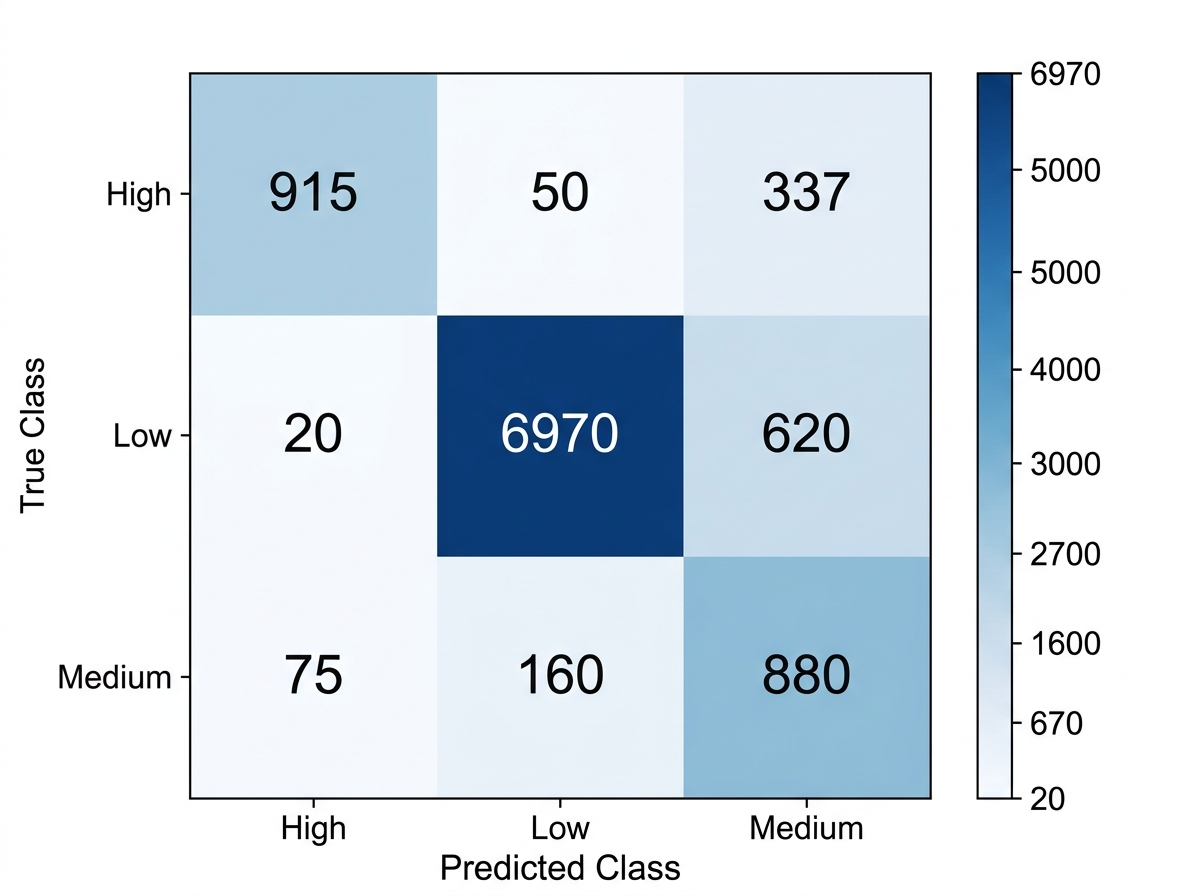
\includegraphics[width=0.88\linewidth]{figures/fig3_confusion_matrix.jpg}
\caption{Confusion Matrix for the Deployed Informer Model ($N = 10,027$).}
\label{fig:cm_informer}
\end{figure}

\subsection{Training Time Analysis}
Computational efficiency during training is essential for grid deployment scalability. Table \ref{tab:training_time} compares total execution time over 50 epochs across key deep learning architectures.

\begin{table}[htbp]
\caption{Training Time Comparison Across Key Architectures (50 Epochs)}
\centering
\resizebox{\columnwidth}{!}{%
\begin{tabular}{lc}
\toprule
\textbf{Model Architecture} & \textbf{Total Training Execution Time (Seconds)} \\
\midrule
\textbf{Informer (Primary)} & \textbf{111.20 s} \\
GRU & 149.85 s \\
LSTM & 168.27 s \\
TimesNet & 318.47 s \\
TFT & 332.51 s \\
PatchTST & 357.63 s \\
\bottomrule
\end{tabular}%
}
\label{tab:training_time}
\end{table}

Informer trained in 111.20 seconds, delivering a 3x speedup over TFT (332.51 s) and PatchTST (357.63 s) due to its ProbSparse attention mechanism.

\subsection{Statistical Validation}
To test whether accuracy differences among top models are statistically significant, we conducted paired McNemar's test ($\chi^2$) and Wilcoxon signed-rank tests across 10,027 test windows under significance threshold $\alpha = 0.05$.

Table \ref{tab:stat_tests} presents hypothesis test results. The null hypothesis ($H_0$: identical prediction performance) cannot be rejected for Informer vs. GRU ($p = 0.1166$), Informer vs. XGBoost ($p = 0.4756$), or Informer vs. Random Forest ($p = 0.8958$). Statistical significance ($p < 0.05$) was established only for Informer vs. TimesNet ($p = 0.0165$).

\begin{table}[htbp]
\caption{Pairwise Statistical Hypothesis Test Results ($\alpha = 0.05$)}
\centering
\resizebox{\columnwidth}{!}{%
\begin{tabular}{lcccc}
\toprule
\textbf{Comparison Pair} & \textbf{McNemar $\chi^2$} & \textbf{McNemar $p$} & \textbf{Wilcoxon $p$} & \textbf{Significance Status} \\
\midrule
Informer vs GRU & 2.463 & 0.1166 & 0.1036 & Not Significant ($p \ge 0.05$) \\
Informer vs XGBoost & 0.509 & 0.4756 & 0.4485 & Not Significant ($p \ge 0.05$) \\
Informer vs RF & 0.017 & 0.8958 & 0.8442 & Not Significant ($p \ge 0.05$) \\
Informer vs TimesNet & 5.752 & 0.0165 & 0.0138 & Significant ($p < 0.05$) \\
\bottomrule
\end{tabular}%
}
\label{tab:stat_tests}
\end{table}

\subsection{Controlled Feature Ablation}
To quantify the predictive impact of feature subsets, we conducted a controlled feature ablation study training five subset configurations under an accelerated retraining protocol (6 epochs, $lr = 0.002$, Full Model baseline = 88.42\% Accuracy, 77.78\% Macro F1).

As detailed in Table \ref{tab:ablation_results}, removing domain-engineered utilization indicators (\texttt{load\_utilization}, \texttt{demand\_utilization}, \texttt{renewable\_ratio}) produced the largest degradation (-1.56\% Macro F1 drop and -3.28\% Recall drop), confirming the value of domain feature engineering.

\begin{table}[htbp]
\caption{Controlled Ablation Study Performance Comparison}
\centering
\resizebox{\columnwidth}{!}{%
\begin{tabular}{lcccc}
\toprule
\textbf{Experiment Subset} & \textbf{Feat. Count} & \textbf{Accuracy} & \textbf{Macro F1} & \textbf{F1 Drop ($\Delta\%$)} \\
\midrule
Full Model (All Features) & 28 & 88.42\% & 77.78\% & Baseline (0.00\%) \\
-- Weather Variables & 21 & 88.40\% & 76.58\% & -1.53\% \\
-- Temporal Features & 24 & 88.32\% & 76.68\% & -1.41\% \\
-- Engineered Features & 21 & 88.36\% & 76.56\% & -1.56\% \\
Core Features Only & 14 & 88.15\% & 75.42\% & -3.03\% \\
\bottomrule
\end{tabular}%
}
\label{tab:ablation_results}
\end{table}

\subsection{Diurnal Robustness}
To evaluate model performance across daily operational shifts, we partitioned test predictions into four diurnal windows: Peak Hours (18:00--22:00), Off-Peak Hours, Daytime (06:00--17:00), and Nighttime (18:00--05:00).

Table \ref{tab:diurnal_results} shows that Informer exhibits stable performance across diurnal transitions, maintaining 87.29\% accuracy (71.71\% High-Risk recall) during Peak Hours and 87.45\% accuracy (69.84\% High-Risk recall) during Off-Peak Hours.

\begin{table}[htbp]
\caption{Diurnal Operational Performance Comparison}
\centering
\resizebox{\columnwidth}{!}{%
\begin{tabular}{lcccc}
\toprule
\textbf{Diurnal Condition} & \textbf{Model} & \textbf{Accuracy} & \textbf{Macro F1} & \textbf{High-Risk Recall} \\
\midrule
\multirow{3}{*}{Peak Hours (18--22h)} & Informer & 87.29\% & 77.73\% & 71.71\% \\
 & Random Forest & 87.21\% & 78.05\% & 71.38\% \\
 & XGBoost & 87.09\% & 76.27\% & 73.36\% \\
\midrule
\multirow{3}{*}{Off-Peak Hours} & Informer & 87.45\% & 77.65\% & 69.84\% \\
 & Random Forest & 87.44\% & 77.82\% & 69.24\% \\
 & XGBoost & 87.74\% & 76.22\% & 70.24\% \\
\bottomrule
\end{tabular}%
}
\label{tab:diurnal_results}
\end{table}

\subsection{Seasonal Robustness}
We evaluated model stability across three seasonal climatic regimes in Bangladesh: Summer (March--May), Monsoon (June--September), and Winter (November--February).

As presented in Table \ref{tab:seasonal_results} and Fig. \ref{fig:robustness_plots}, High-Risk recall drops across all models during the Summer partition (61.71\% for Informer) compared to Monsoon (91.30\%) and Winter (98.09\%), indicating that intense summer heatwave volatility creates complex load dynamics.

\begin{table}[htbp]
\caption{Seasonal Climatic Regime Performance Comparison}
\centering
\resizebox{\columnwidth}{!}{%
\begin{tabular}{lcccc}
\toprule
\textbf{Season} & \textbf{Model} & \textbf{Accuracy} & \textbf{Macro F1} & \textbf{High-Risk Recall} \\
\midrule
\multirow{3}{*}{Summer (Mar--May)} & Informer & 85.18\% & 76.53\% & 61.71\% \\
 & Random Forest & 84.84\% & 76.28\% & 61.19\% \\
 & XGBoost & 84.31\% & 74.07\% & 62.85\% \\
\midrule
\multirow{3}{*}{Monsoon (Jun--Sep)} & Informer & 91.11\% & 80.33\% & 91.30\% \\
 & Random Forest & 91.71\% & 81.78\% & 91.30\% \\
 & XGBoost & 91.71\% & 81.36\% & 91.30\% \\
\midrule
\multirow{3}{*}{Winter (Nov--Feb)} & Informer & 92.19\% & 72.66\% & 98.09\% \\
 & Random Forest & 92.69\% & 76.14\% & 96.82\% \\
 & XGBoost & 95.76\% & 75.62\% & 96.82\% \\
\bottomrule
\end{tabular}%
}
\label{tab:seasonal_results}
\end{table}

\begin{figure}[htbp]
\centering
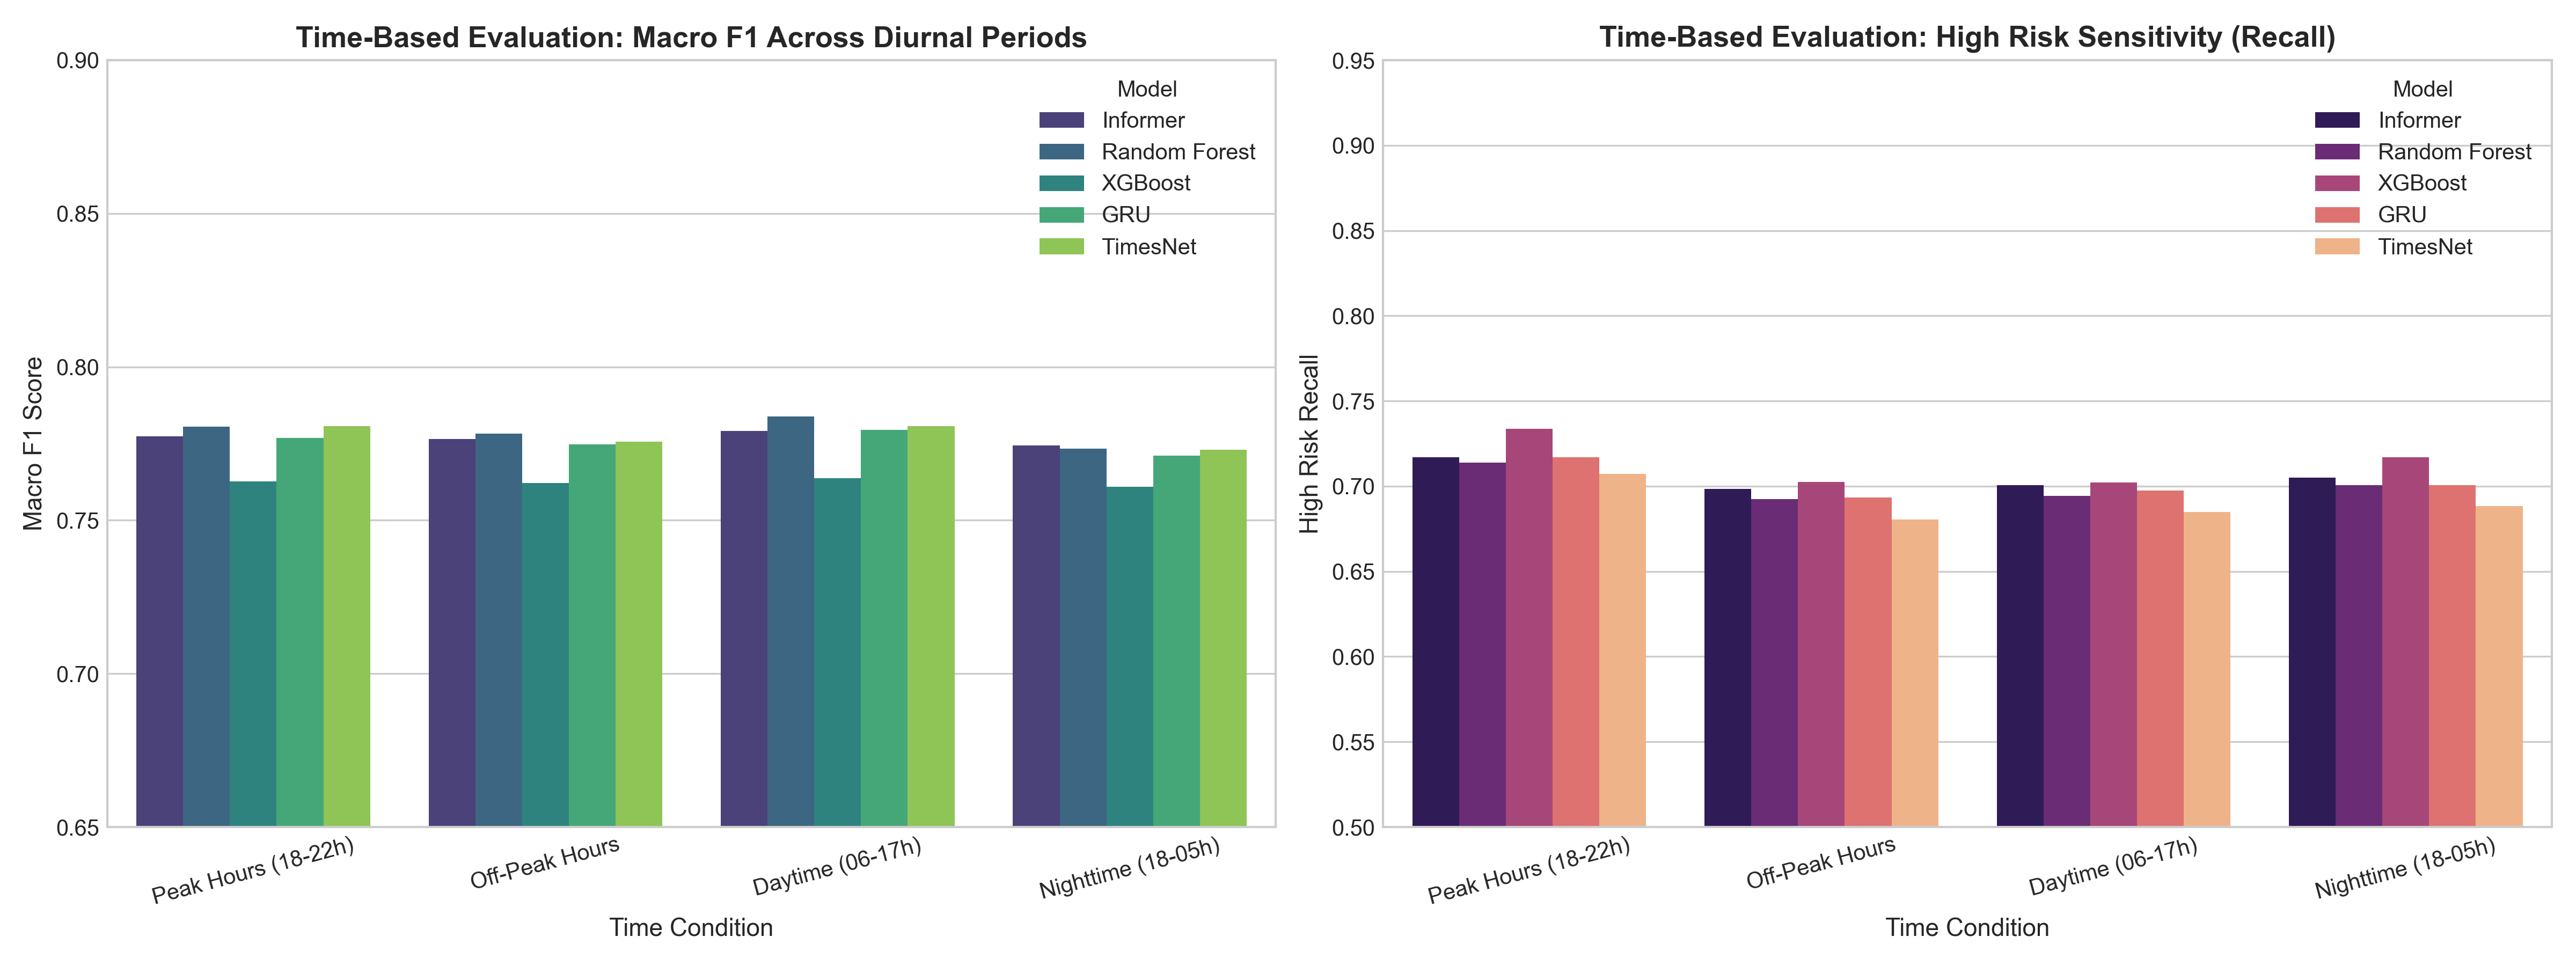
\includegraphics[width=0.88\linewidth]{figures/fig6_diurnal_seasonal_robustness.png}
\caption{Diurnal and Seasonal Robustness Evaluation Profiles.}
\label{fig:robustness_plots}
\end{figure}

\section{Explainability \& Alert Generation}
\subsection{Permutation Feature Importance Analysis}
To provide model interpretability, we evaluated empirical feature importance using permutation-based Macro F1 degradation on the hold-out test split. Features were permuted independently across 10 random iterations.

Fig. \ref{fig:feature_importance} illustrates the top feature importances for Informer. Engineered utilization indicators (\texttt{load\_utilization} and \texttt{demand\_utilization}) account for 74.29\% of the observed performance degradation when permuted, confirming that capacity stress variables are the primary drivers of model predictions. Electrical and asset telemetry (\texttt{transformer\_load}, \texttt{electricity\_demand}) account for 24.39\%, while meteorological variables (\texttt{temperature}, \texttt{rainfall}, \texttt{humidity}) contribute 1.97\%, and temporal flags account for 0.17\%. This confirms that environmental variables act as secondary stress modifiers operating through thermal indices ($\text{THI}$).

\begin{figure}[htbp]
\centering
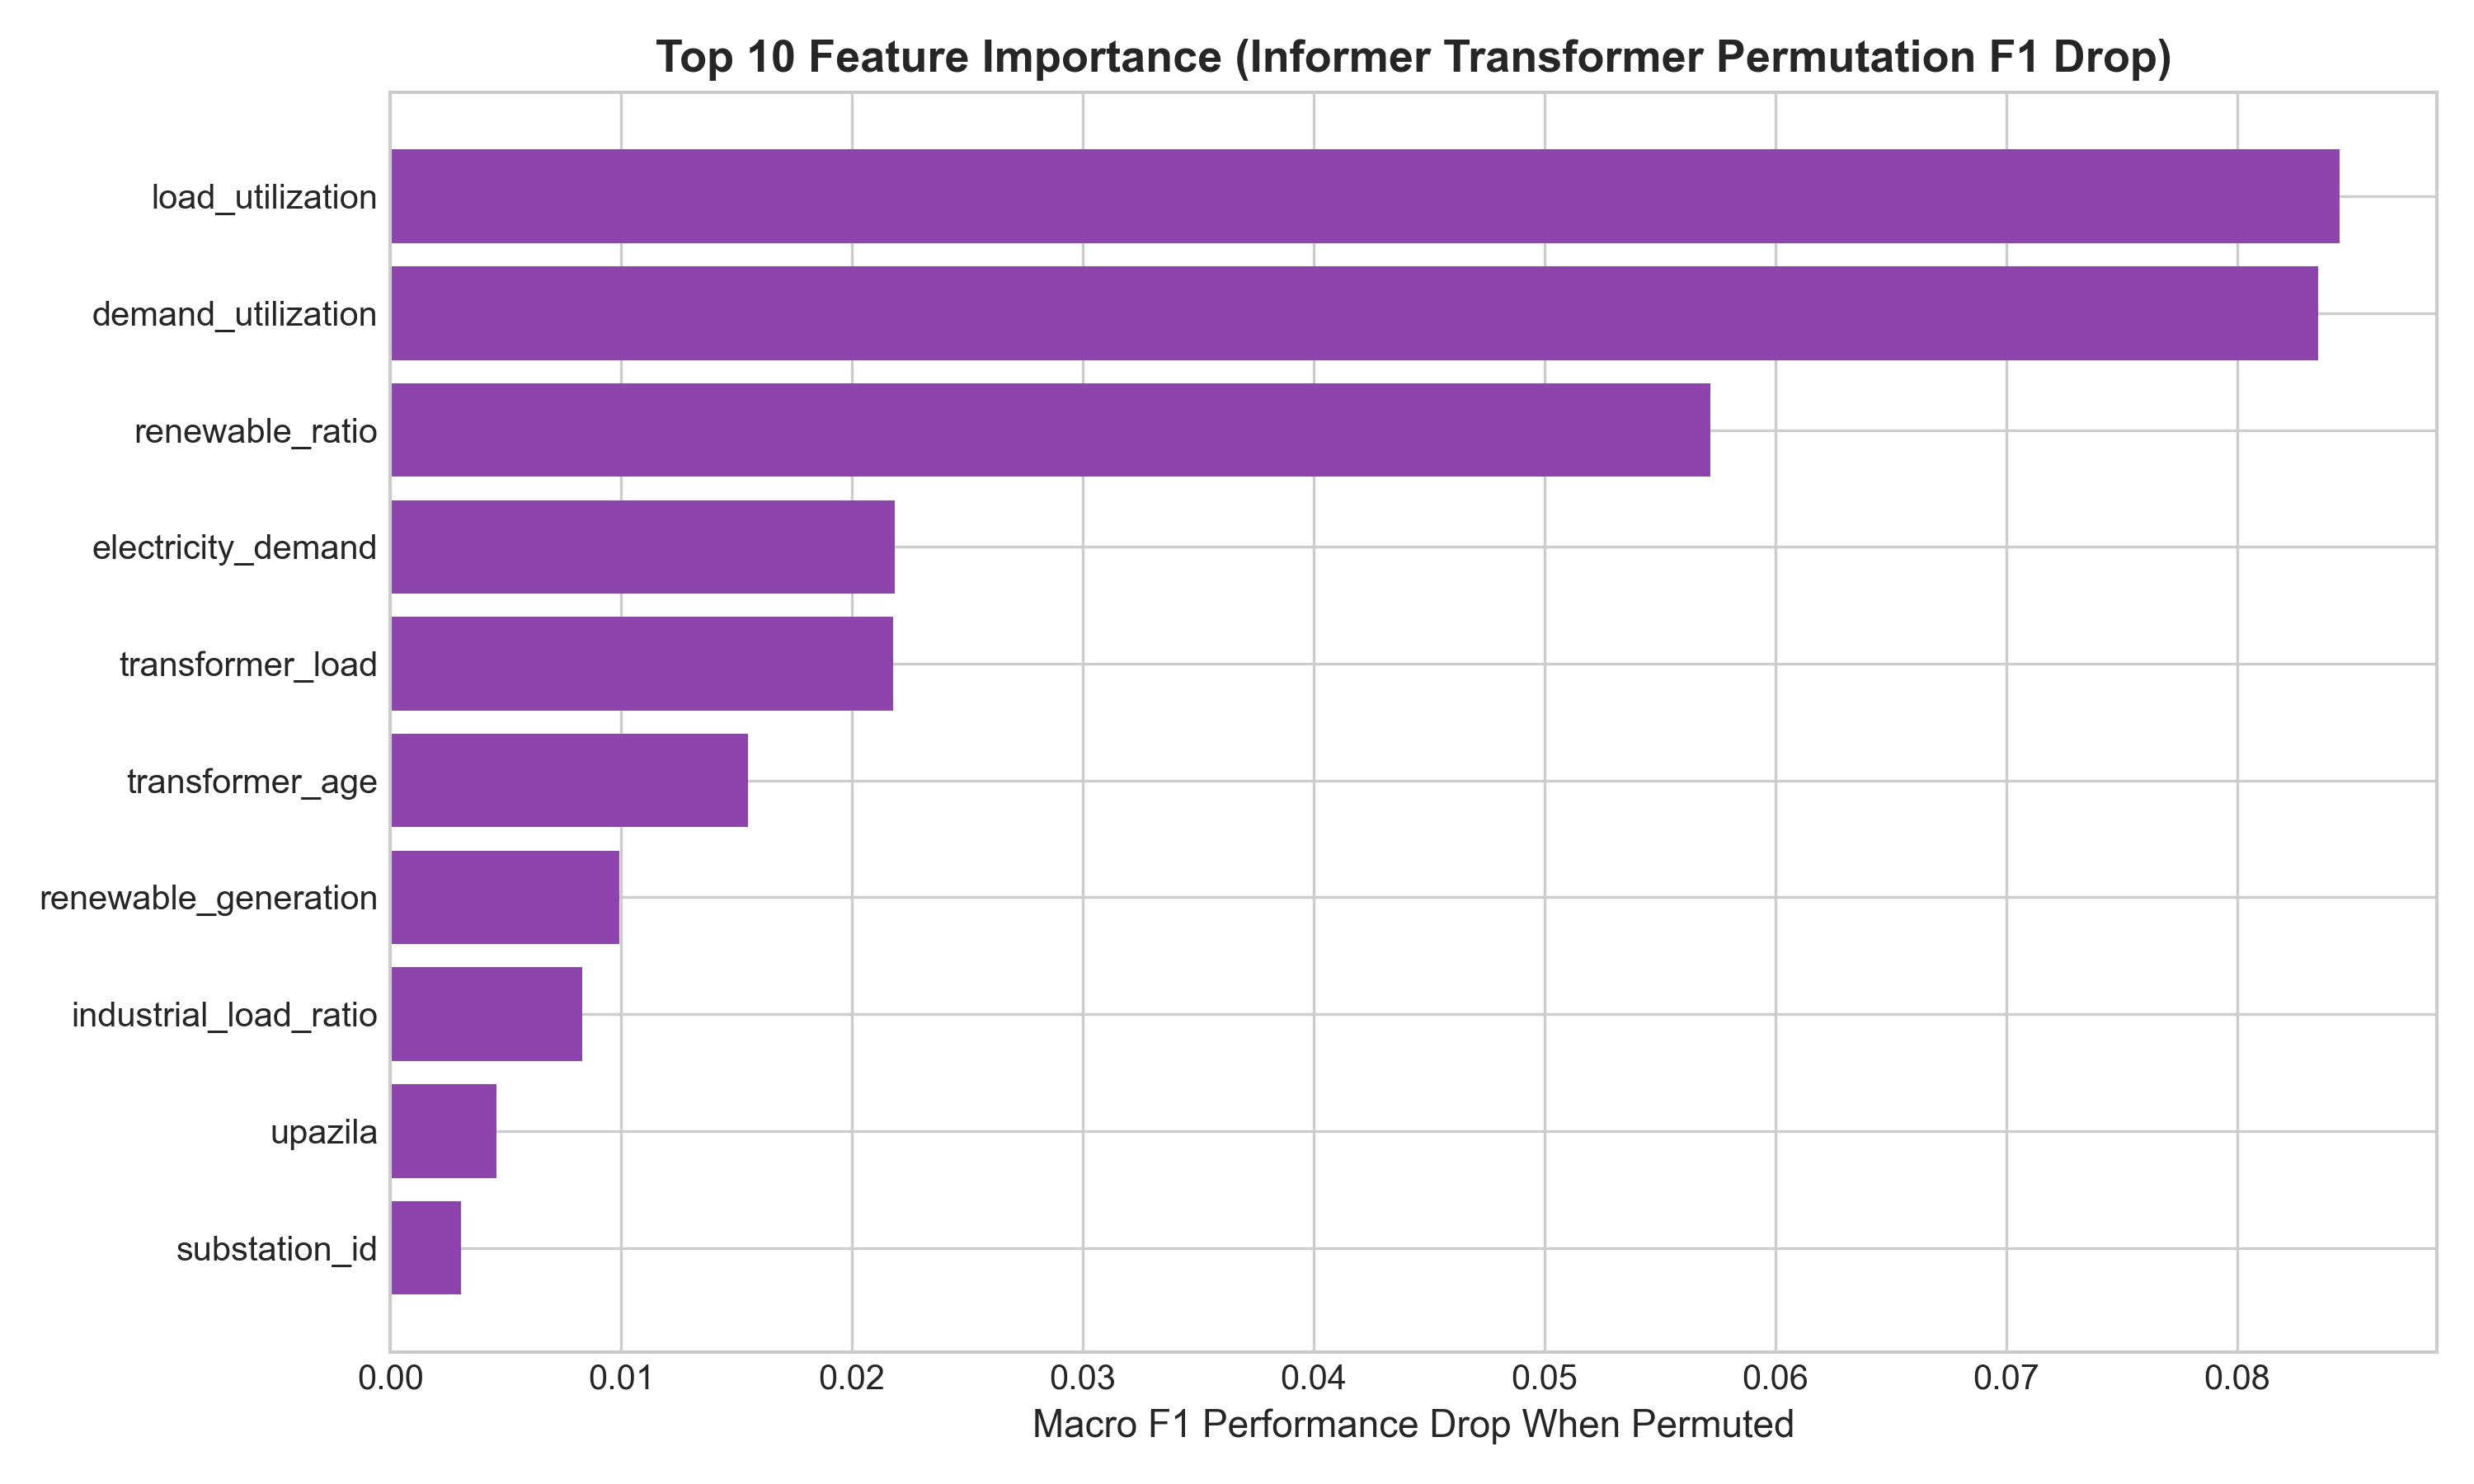
\includegraphics[width=0.88\linewidth]{figures/fig4_feature_importance.png}
\caption{Permutation Feature Importance Profile for the Informer Model.}
\label{fig:feature_importance}
\end{figure}

\subsection{Rule-Based Intelligent Alert Generation Engine}
To bridge deep learning probability outputs with utility control room operations, SmartGrid Sentinel routes model Softmax probabilities through a Rule-Based Natural Language Explanation Engine. Rather than providing uninterpretable raw attribution scores, the rule engine evaluates input telemetry against physical grid operating thresholds:

\begin{itemize}
    \item \textbf{GREEN (Normal Operation):} Predicted Risk = \texttt{Low}. Transformer loading is within safe operating bounds ($U_{\text{load}} \le 0.75$). Normal grid dispatch continues.
    \item \textbf{YELLOW (Warning Advisory):} Predicted Risk = \texttt{Medium}. Transformer loading is moderate ($0.75 < U_{\text{load}} \le 0.85$). The rule engine issues operator advisories: \textit{``Moderate capacity stress detected on feeder transformer. Dispatchers should monitor demand growth and notify industrial loads.''}
    \item \textbf{RED (Urgent Emergency):} Predicted Risk = \texttt{High}. Severe transformer loading ($U_{\text{load}} > 0.85$). The rule engine issues urgent advisories: \textit{``Electricity demand exceeds capacity thresholds ($U_{\text{load}} > 0.85$), indicating severe overload risk. Initiate precautionary load shedding on non-essential commercial feeders.''}
\end{itemize}

If environmental heat stress is high ($\text{THI} > 28.0$), the module appends: \textit{``Elevated environmental heat stress detected ($\text{THI} > 28.0$), accelerating transformer thermal degradation risks.''} These advisories are coupled with citizen recommendations (e.g., charging essential devices, throttling high-power cooling appliances).

\section{Deployment Architecture}
The production backend for SmartGrid Sentinel is implemented as a lightweight RESTful web service using FastAPI (\texttt{backend/app.py}). The API exposes endpoints for real-time telemetry ingestion, sequence window transformation, model inference, and rule-based alert generation.

\begin{enumerate}
    \item \textbf{Telemetry Ingestion \& Payload Parsing:} Incoming JSON requests containing historical 5-step telemetry arrays are validated against schemas specifying 27 raw input fields per timestamp.
    \item \textbf{Sequence Scaling \& Inference:} The backend applies pre-fitted \texttt{StandardScaler} parameters to transform sequence arrays ($X \in \mathbb{R}^{1 \times 5 \times 28}$) before executing a forward pass on pre-trained checkpoint \texttt{epoch\_10.pth}.
    \item \textbf{Softmax Probability Computation:} Output logits are converted to normalized Softmax probabilities ($\sum p_i = 1.0000$) to determine predicted risk levels.
    \item \textbf{Rule Parser \& Advisory Ingestion:} Risk levels and physical telemetry parameters ($U_{\text{load}}$, $\text{THI}$) are processed through the rule engine to yield color-coded alert flags (\texttt{GREEN}, \texttt{YELLOW}, \texttt{RED}) and natural language action checklists.
    \item \textbf{API Fault Tolerance \& Exception Handling:} Automated exception handlers catch malformed JSON payloads or unknown Upazila IDs, returning HTTP 400 (Bad Request) and HTTP 422 (Unprocessable Entity) status codes without process failure.
\end{enumerate}

\section{Discussion}
\subsection{Comparative Model Interpretation}
Informer was retained as the primary sequence model for production deployment based on its observed benchmark performance, low catastrophic High-to-Low missed alert count (50 cases / 4.48\%), training loss stability across 50 epochs, and $O(L \log L)$ computational efficiency. Pairwise statistical testing confirmed that overall accuracy differences between Informer and top-performing architectures (GRU, XGBoost, Random Forest) were not statistically significant ($p = 0.1166$ vs. GRU, $p = 0.4756$ vs. XGBoost, $p = 0.8958$ vs. Random Forest). Rather than claiming absolute statistical dominance, Informer was selected because its ProbSparse attention mechanism scales efficiently to longer sequence lookbacks ($O(L \log L)$) while training 3x faster than PatchTST and TFT without validation loss divergence.

\subsection{High-Risk Error Behavior}
Analyzing error patterns reveals critical operational trade-offs across model families. Although XGBoost achieved competitive accuracy (87.58\%), it produced 128 catastrophic High-to-Low missed alerts ($11.48\%$ of High-Risk test cases). Informer limited catastrophic High-to-Low errors to 50 cases ($4.48\%$). Misclassifications occur predominantly along continuous boundary conditions where transformer load is between 75\% and 85\% accompanied by rapid localized rainfall spikes.

\subsection{Feature Importance \& Explainability Interpretation}
Empirical permutation feature importance demonstrates that domain-engineered utilization indicators (\texttt{load\_utilization} and \texttt{demand\_utilization}) account for over 74\% of Informer's predictive contribution. Meteorological variables (\texttt{temperature}, \texttt{rainfall}, \texttt{humidity}) exhibit lower direct permutation impact but influence predictions through thermal stress indices ($\text{THI}$) and utilization ratios.

\subsection{Condition-Dependent Performance}
Robustness evaluations across operating conditions confirm model stability across diurnal cycles (Peak Hours accuracy 87.29\% vs. Off-Peak 87.45\% for Informer). Seasonally, all evaluated models exhibit lower High-Risk recall during Summer (61.71\% for Informer) compared to Monsoon (91.30\%) and Winter (98.09\%), indicating that severe summer heatwaves create complex load volatility that warrants continuous monitoring.

\subsection{Practical Implications for Grid Operators}
Linking sequence predictions with a physical threshold rule engine bridges the gap between deep learning probability outputs and control room operations. By pairing tri-level risk scores with human-readable explanations and action checklists, dispatchers can initiate precautionary load shifting before automated circuit breakers trip, transitioning grid management from reactive load shedding to predictive contingency planning.

\section{Threats to Validity}
\subsection{Internal Validity}
Internal validity concerns potential experimental biases during data curation, feature engineering, or model training. We mitigated temporal data leakage by enforcing chronological train-test splits (80/20 per feeder stream) without random shuffling or K-fold cross-validation. Preprocessing parameters for feature scaling (\texttt{StandardScaler}) were computed strictly on the training partition. Furthermore, target shifting was performed per feeder stream prior to sequence generation.

\subsection{External Validity}
External validity addresses the generalizability of results across different distribution networks. The telemetry dataset spans 143 Upazilas across 15 districts in Sylhet and Chattogram divisions. While this provides diverse coverage across tropical coastal and hilly regions in Bangladesh, operational dynamics in other geographical regions or distribution utilities with different industrial load ratios may exhibit distinct demand profiles.

\subsection{Construct Validity}
Construct validity relates to whether evaluation metrics accurately capture real-world grid performance. We evaluated models across multiple complementary dimensions, including One-vs-Rest Macro F1, Weighted F1, Accuracy, Macro ROC-AUC, Macro PR-AUC, catastrophic High-to-Low missed alert counts, and training execution time, ensuring a holistic assessment.

\section{Limitations}
While SmartGrid Sentinel provides a robust, interpretable forecasting framework, several limitations should be noted:
\begin{enumerate}
    \item \textbf{Geographic Scope:} Telemetry data were collected from 143 Upazilas across 15 districts in Sylhet and Chattogram divisions. Nationwide grid deployment will require ingesting telemetry from all 495 Upazilas across Bangladesh.
    \item \textbf{Single-Step Forecast Horizon:} The current system evaluates a single 2-hour ahead forecast step ($T+2\text{h}$). Multi-horizon forecasts ($T+4\text{h}$, $T+6\text{h}$) are necessary for long-term generation scheduling.
    \item \textbf{Substation Network Topology:} Telemetry streams are processed per feeder without explicit topological graph modeling of inter-substation transmission lines.
\end{enumerate}

\section{Conclusion and Future Work}
SmartGrid Sentinel establishes a localized, 2-hour ahead load-shedding risk forecasting framework for electricity distribution networks in Bangladesh. Evaluating 12 candidate architectures across 65,983 telemetry snapshots (143 Upazilas, 1,000 feeders), the Informer sequence model achieved an overall accuracy of 87.41\%, a Macro F1-score of 77.68\%, and a Weighted F1-score of 88.44\% on 10,027 test sequence windows, limiting catastrophic High-to-Low missed alerts to 50 cases (4.48\%). Paired statistical testing (McNemar and Wilcoxon tests) confirmed that performance differences between Informer and top models (GRU, XGBoost, Random Forest) are not statistically significant ($p \ge 0.05$), justifying Informer's selection based on training stability, error behavior, and $O(L \log L)$ efficiency (111.20 s over 50 epochs). Controlled feature ablation verified the importance of domain utilization indicators, while robustness analysis revealed seasonal performance shifts during summer heatwaves. Routing predictions through a physical threshold rule engine converts risk probabilities into actionable control room advisories.

Future work will focus on:
\begin{enumerate}
    \item Extending predictions to multi-step forecast horizons ($T+4\text{h}$, $T+6\text{h}$) to support long-term generation scheduling.
    \item Incorporating Graph Neural Networks (GNNs) and Spatial-Temporal Graph Convolutional Networks (ST-GCNs) to model physical substation network topology and inter-feeder power transfers.
    \item Expanding telemetry collection to cover all 495 Upazilas across Bangladesh for nationwide grid deployment.
\end{enumerate}


\clearpage
\bibliographystyle{IEEEtran}
\bibliography{references}

\end{document}
